% -*- TeX:de -*-
\NeedsTeXFormat{LaTeX2e}
\documentclass[12pt,a4paper]{article}
\usepackage[german]{babel} % german text
\usepackage[DIV12]{typearea} % size of printable area
\usepackage[T1]{fontenc} % font encoding
%\usepackage[latin1]{inputenc} % most likely on Windows
\usepackage[utf8]{inputenc} % probably on Linux
\usepackage{multicol}

% PLOTTING
\usepackage{pgfplots} 
\usepackage{pgfplotstable}
\usepackage{url}
\usepackage{graphicx} % to include images
\usepackage{tikz}
\usepackage{subfigure} % for creating subfigures
\usepackage{amsmath} % a bunch of symbols
\usepackage{amssymb} % even more symbols
\usepackage{booktabs} % pretty tables

% a floating environment for circuits
\usepackage{float}
\usepackage{caption}

%\newfloat{circuit}{tbph}{circuits}
%\floatname{circuit}{Schaltplan}

% a floating environment for diagrams
%\newfloat{diagram}{tbph}{diagrams}
%\floatname{diagram}{Diagramm}

\selectlanguage{german} % use german

\begin{document}

%%%%%%% DECKBLATT %%%%%%%
\thispagestyle{empty}
			\begin{center}
			\Large{Fakultät für Physik}\\
			\end{center}
\begin{verbatim}


\end{verbatim}
							%Eintrag des Wintersemesters
			\begin{center}
			\textbf{\LARGE WS 2013/14}
			\end{center}
\begin{verbatim}


\end{verbatim}
			\begin{center}
			\textbf{\LARGE{Physikalisches Praktikum\\ für das Bachelorstudium}}
			\end{center}
\begin{verbatim}




\end{verbatim}

			\begin{center}
			\textbf{\LARGE{PROTOKOLL}}
			\end{center}
			
\begin{verbatim}





\end{verbatim}

			\begin{flushleft}
			\textbf{\Large{Experiment (Nr., Titel):}}\\
							%Experiment Nr. und Titel statt den Punkten eintragen
			\LARGE{PW3 Elastizität / Trägheitsmoment}	
			\end{flushleft}

\begin{verbatim}

\end{verbatim}	
							%Eintragen des Abgabedatums, oder des Erstelldatums des Protokolls
			\begin{flushleft}
			\textbf{\Large{Datum:}} \Large{24.10.2013}
			\end{flushleft}
			
\begin{verbatim}
\end{verbatim}
							%Namen der Protokollschreiber
		\begin{flushleft}
			\textbf{\Large{Namen:}} \Large{Patrick Braun, Johannes Kurz}
			\end{flushleft}

\begin{verbatim}


\end{verbatim}
							%Kurstag und Gruppennummer, zb. Fr/5
			\begin{flushleft}
			\textbf{\Large{Kurstag/Gruppe:}} \Large{DO/2}
			\end{flushleft}

\begin{verbatim}



\end{verbatim}
							%Name des Betreuers, das Praktikum betreute.
			\begin{flushleft}
			\LARGE{\textbf{Betreuer:}}	\Large{Franz Sachslehner}	
			\end{flushleft}

%%%%%%% DECKBLATT ENDE %%%%%%%
\pagebreak
\setlength{\columnsep}{20pt}
\begin{multicols}{2}
\section{Einleitung}
PW3 dreht sich inhaltlich um eine Einführung in die Messung von Materialeigenschaften, sowie um Rotationsbewegungen, vor allem um das Trägheitsmoment.\\
Das verbindende Element der beiden Aufgabenteile ist jedoch das didaktische Thema der Einheit: eine erste Erfahrung im Umgang mit computergestützter Messdatenerfassung und der Weiterverarbeitung dieser Roh-Daten.\\
Den tatsächlichen Versuchsaufbauten entsprechend, ist dieses Protokoll in 3 Teile gegliedert:\\
- Elastizität von Aluminium\\
- Torsion von Aluminium\\
- Trägheitsmoment eines Pendels mit Zusatzmasse

\section{Elastizität}

In diesem Versuch soll der Elastizitätsmodul E von Aluminium bestimmt werden.\\
Er beschreibt den (für kleine Spannungen) linearen Zusammenhang zwischen der Spannung, die auf ein Objekt wirkt, und der daraus resultierenden Dehnung. Er ist eine Konstante und eine Materialeigenschaft.\\
Metalle besitzen einen elastischen sowie einen plastischen Bereich: Kehrt das untersuchte Metall, nachdem die ausgeübte Spannung wieder weggenommen wurde, in seine ursprüngliche Form zurück, spricht man vom \textit{elastischen Bereich} der Spannungs-Dehnungskurve.\\
Bei höheren Spannungen bleibt eine gewisse Verformung zurück, auch wenn keine Kraft mehr auf das Metall ausgeübt wird; man spricht vom \textit{plastischen Bereich}.


\subsection{Versuchsaufbau und \\-durchführung}
Equipment:\\
Eine Zugmaschine mit Verstärker (Fa. INSTRON)\\
Ein Voltmeter FLUKE 175\\
Ein Aluminiumdraht\\
Eine Mikrometerschraube\\
Eichgewichte\\
Zwei Messinglehren; (100 $\pm$ 0.1) mm\\
\\
\\
Der Aluminiumdraht wird in den Lastrahmen der Zugmaschine eingespannt (Abb. 2.1). Der Abstand zwischen den beiden Klemmen beträgt (100 $\pm$ 0.1) mm. Er wird mit Hilfe der beiden Messinglehren erreicht.\\
% !!! fig 2.1 Skizze des Versuchs einfügen %%%%%%%%%%%%%
Die untere Klemme sitzt auf einem beweglichen Rahmen, der nach Beginn des Versuches mit 0.5 mm/min nach unten fährt. Dabei sendet die Kraftmesszelle im oberen Teil der Zugmaschine eine Spannung, proportional zur Kraft, die auf den Draht wirkt, an die Verstärkereinheit und über einen A/D-Wandler in den PC zur Aufzeichnung.\\
Das Signal wird in $[V]$ aufgezeichnet.\\
Daher muss die Datenausgabe vor Versuchsbeginn kalibriert werden:\\
Es werden 2 kg der Eichgewichte an der obere Klemme angebracht, und der Verstärker wird, mit Hilfe des Voltmeters) so eingestellt, dass 40mV ausgegeben werden:\\
$0.04 V \equiv 2 kg * 9.81 m/s^2 $\\
\\
Damit ergibt sich ein Umrechnungsfaktor von $1V \equiv 490,5 N $.\\
Schließlich muss die gemessene Kraft in Spannung umgerechnet werden durch $\sigma = \frac{F}{q}$, wobei q der Querschnitt des Drahtes ist.\\
Die aufgezeichnete Zeit wird durch\\
$ \epsilon = \frac{v*t}{L_{0}} $\\
in die Dehnung $\epsilon$ konvertiert, wobei die Geschwindigkeit des Zugrahmens\\
 $v = 0.5 mm/min$ und die Ausgangslänge $ L_{0} = (100 \pm 0.1) mm $.\\
\\
Die so gewonnenen Daten werden in einem Diagramm Spannung gegen Dehnung aufgetragen.\\
Es wird ein linearer Anstieg im Elastizitätsbereich erwartet, dessen Steigung im linearen Fit direkt den E-Modul ergibt.\\

%"Für eine genauere Anleitung zur Versuchdurchführung siehe www....anfpra/pw3 %%%% ????


\subsection{Messdaten und Ergebnisse}
Dicke des Aluminium-Drahtes [mm]:\\
$(1,98\pm 0.01)$mm\\
\\
(gemessen an 5 Stellen, gleichmäßig verteilt:
1.98
1.98
1.98
1.99
1.98\\
die Standardabw. des Mittelwerts ist trotz Student-t-Korrektur kleiner als die Auflösung des Messgerätes)\\

%Voltmeter am Verstärker pendelt zwischen 9.98mV ohne Gewicht. Mit 2kg Last bei $(40 \pm 0.1)$mV. 



\section{Torsionspendel}
In diesem Teil von PW3 soll nun der Torsionsmodul G von Aluminium bestimmt werden. Aus diesem und dem in Kapitel 2 ermittelten Elastizitätsmodul E kann schließlich die Poissonzahl $\nu $ berechnet werden.\\
\subsection{Versuchsaufbau und \\-durchführung}
Equipment:\\
Ein Torsionspendel, bestehend aus einer Querstange, montiert an einem Aluminiumdraht\\
Ein Satz Gewichte (je 2 gleiche)\\
Eine Mikrometerschraube\\
Ein Maßband\\
Eine Stoppuhr\\
Eine Waage\\
% !!!! bitte markennahmen, evtl auflösung/genauigkeit einfügen
\\
\\
Das Pendel wird aufgebaut, wie in Abb. 3.1.\\
% !!!!!! skizze 3.1 einfügen... zeichnung - torsionspendel
2 gleiche Massen werden in gleichem Abstand l von der Mitte befestigt. Anschließend wird das Pendel derartig in Bewegung versetzt, dass die Querstange in der Ebene um ihre Ruhelage, also normal zum Aluminiumdraht, oszilliert. Der Draht erfährt also eine Scherung.\\
Es ist darauf zu achten, dass die Bewegung möglichst gleichmäßig und rund läuft. Eine nahezu saubere Torsion des Drahtes, ohne Verzerrungen, ist in dieser Art der Durchführung (von Hand) kaum möglich, einige Übungsläufe vor der ersten Messung können jedoch eindeutige Verbesserungen der Schwingung erwirken.\\
Mit der Stoppuhr wird die Dauer mehrerer Schwingungsperioden gemessen. Die Messung mehrerer Perioden bewirkt, dass der einigermaßen konstante Fehler durch die Ungenauigkeit beim Messen von Hand, geteilt wird und sein Einfluss auf einen einzelnen Durchgang damit wesentlich verringert wird.\\
Außerdem sollte beim Nulldurchgang, also dem Moment größter kinetischer Energie des Pendels gemessen werden. Eine Markierung des Nulldurchgangs unter dem ruhenden Pendel kann auch helfen, die Messung zu verbessern.\\
Der Torsionsmodul berechnet sich durch\\
$$G = \frac{2LD}{\pi r^4}$$
wobei L die Länge des Drahtes und D die Winkelrichtgröße ist.\\
Diese lässt sich aus dem Steiner'schen Satz durch Elimination mit 2 Messungen mit verschiedenem Abstand l (Entfernung der Massen vom Mittelpunkt) und damit 2 verschiedenen Periodendauern T ausdrücken:\\
$$ D=8\pi ^2 m* \frac{l_1^2-l_2^2}{T_1^2-T_2^2}$$
Aus beiden Gleichungen wird also G berechnet.\\
Zuletzt wird die Poissonzahl $\nu$, die das Verhältnis zwischen Änderung der Länge und des Durchmessers eines Festkörpers unter Spannung beschreibt, errechnet durch:\\
$$ \nu = \frac{E}{2G}-1$$


\subsection{Messdaten und Ergebnisse}

%\begin{figure}[H]
%	\centering
%  	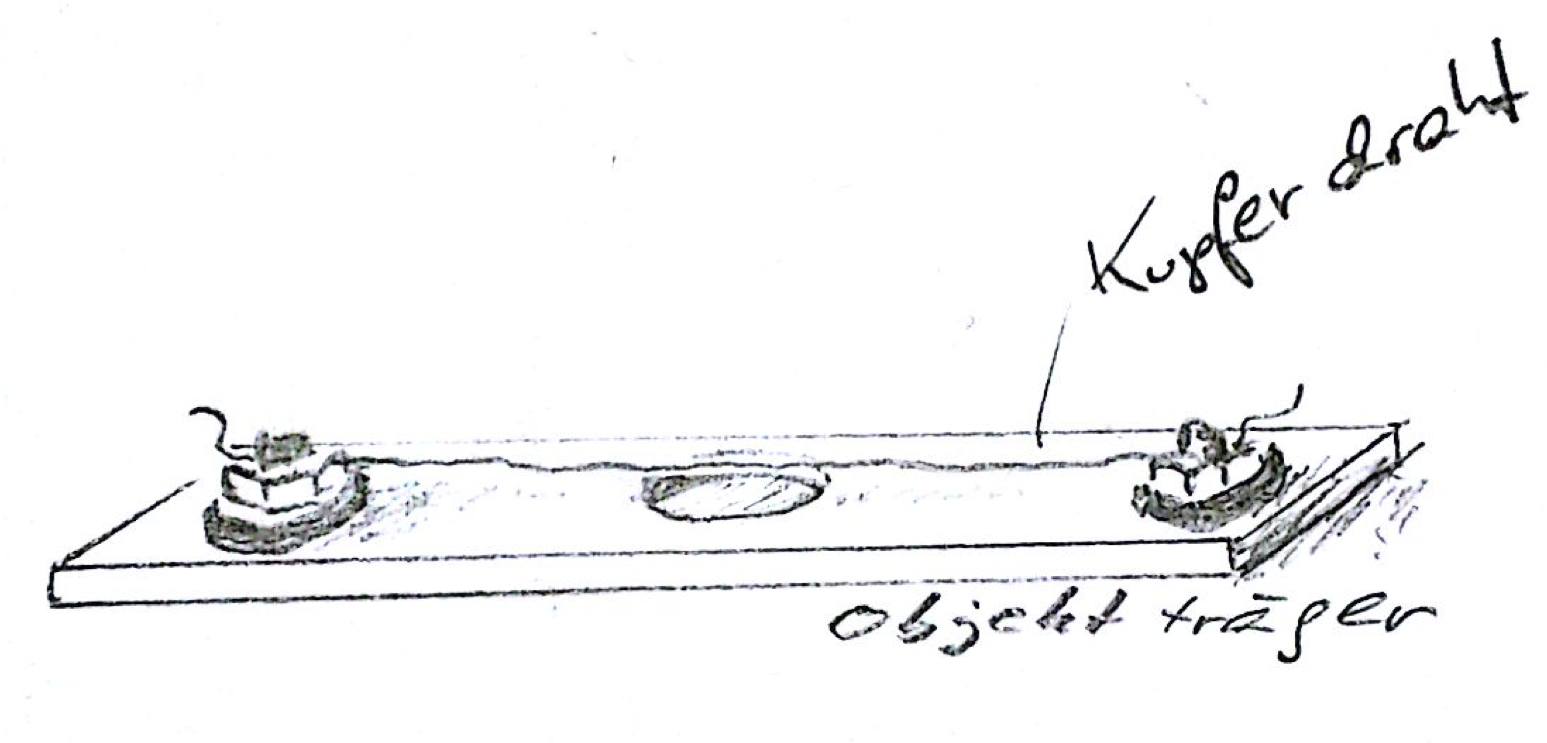
\includegraphics[scale=0.3]{./figure/draht.png}
%	\caption{Drahtprobe auf Objektträger}
%	\label{fig:201}
%\end{figure}

\section{Pendel}
In diesem Versuch soll das gesamte , sowie die einzelnen Teilträgheitsmomente eines physikalischen Pendels, bestehend aus einem Rad und einem daran montierten Zylinder, ermittelt werden.\\
Dazu wird der Steiner'sche Satz benutzt, der die Trägheitsmomente mehrerer Objekte mit parallelen 

Messen der Trägheit

\end{document}